\section{Overview}\label{sec:overview}
In this section, we provide an overview of the entire paper and proposed RL system for general bipedal locomotion control, as illustrated in Fig.~\ref{fig:overview}. 
We first provide an introduction of the importance of utilizing the robot's I/O history in the locomotion control in Sec.~\ref{sec:background}. In this section, we showcase that the robot's long I/O history can enable system identification and state estimations during real-time control, from both control and RL perspectives.
This results in the design of the backbone of this work: a new control architecture that utilizes a dual-history of both the bipedal robot's long-term and short-term I/O history, which is presented in Sec.~\ref{sec:controller}. 
Specifically, such a control architecture does not only utilize the long history but also exploits explicit short history of the robot.
The proposed dual-history structure enables effective use of robot's history, as the long history brings adaptivity (validated in Sec.~\ref{subsec:adaptivity}) and the short history complements the use of long history by enabling better real-time control (substantiated in Sec.~\ref{sec:policy_structure}). 
This control policy, which is represented by a deep neural network, is optimized by model-free RL in Sec.~\ref{sec:training}.
Since this paper aims to develop a controller that is capable of accomplishing diverse tasks using highly dynamic locomotion skills, the training in Sec.~\ref{sec:training} is characterized by multi-stage training in simulation. 
This training strategy provides a structured curriculum, starting with a single-task training where the robot focuses on a fixed task, followed by task randomization that diversifies the tasks the robot is trained on, and concluded by dynamics randomization which alters the dynamics parameters of the robot.
Such a training strategy is able to provide a versatile control policy that can perform a large variety of tasks and zero-shot transferred to the robot hardware.
Furthermore, task randomization can also enhance the robustness of the resulting policy through the generalization among different learned tasks. We show that such robustness results in compliant behaviors to disturbance, which is “orthogonal" to the one brought by dynamics randomization. This is validated in Sec.~\ref{sec:multi_skill}.


\begin{figure}[t]
    \centering
    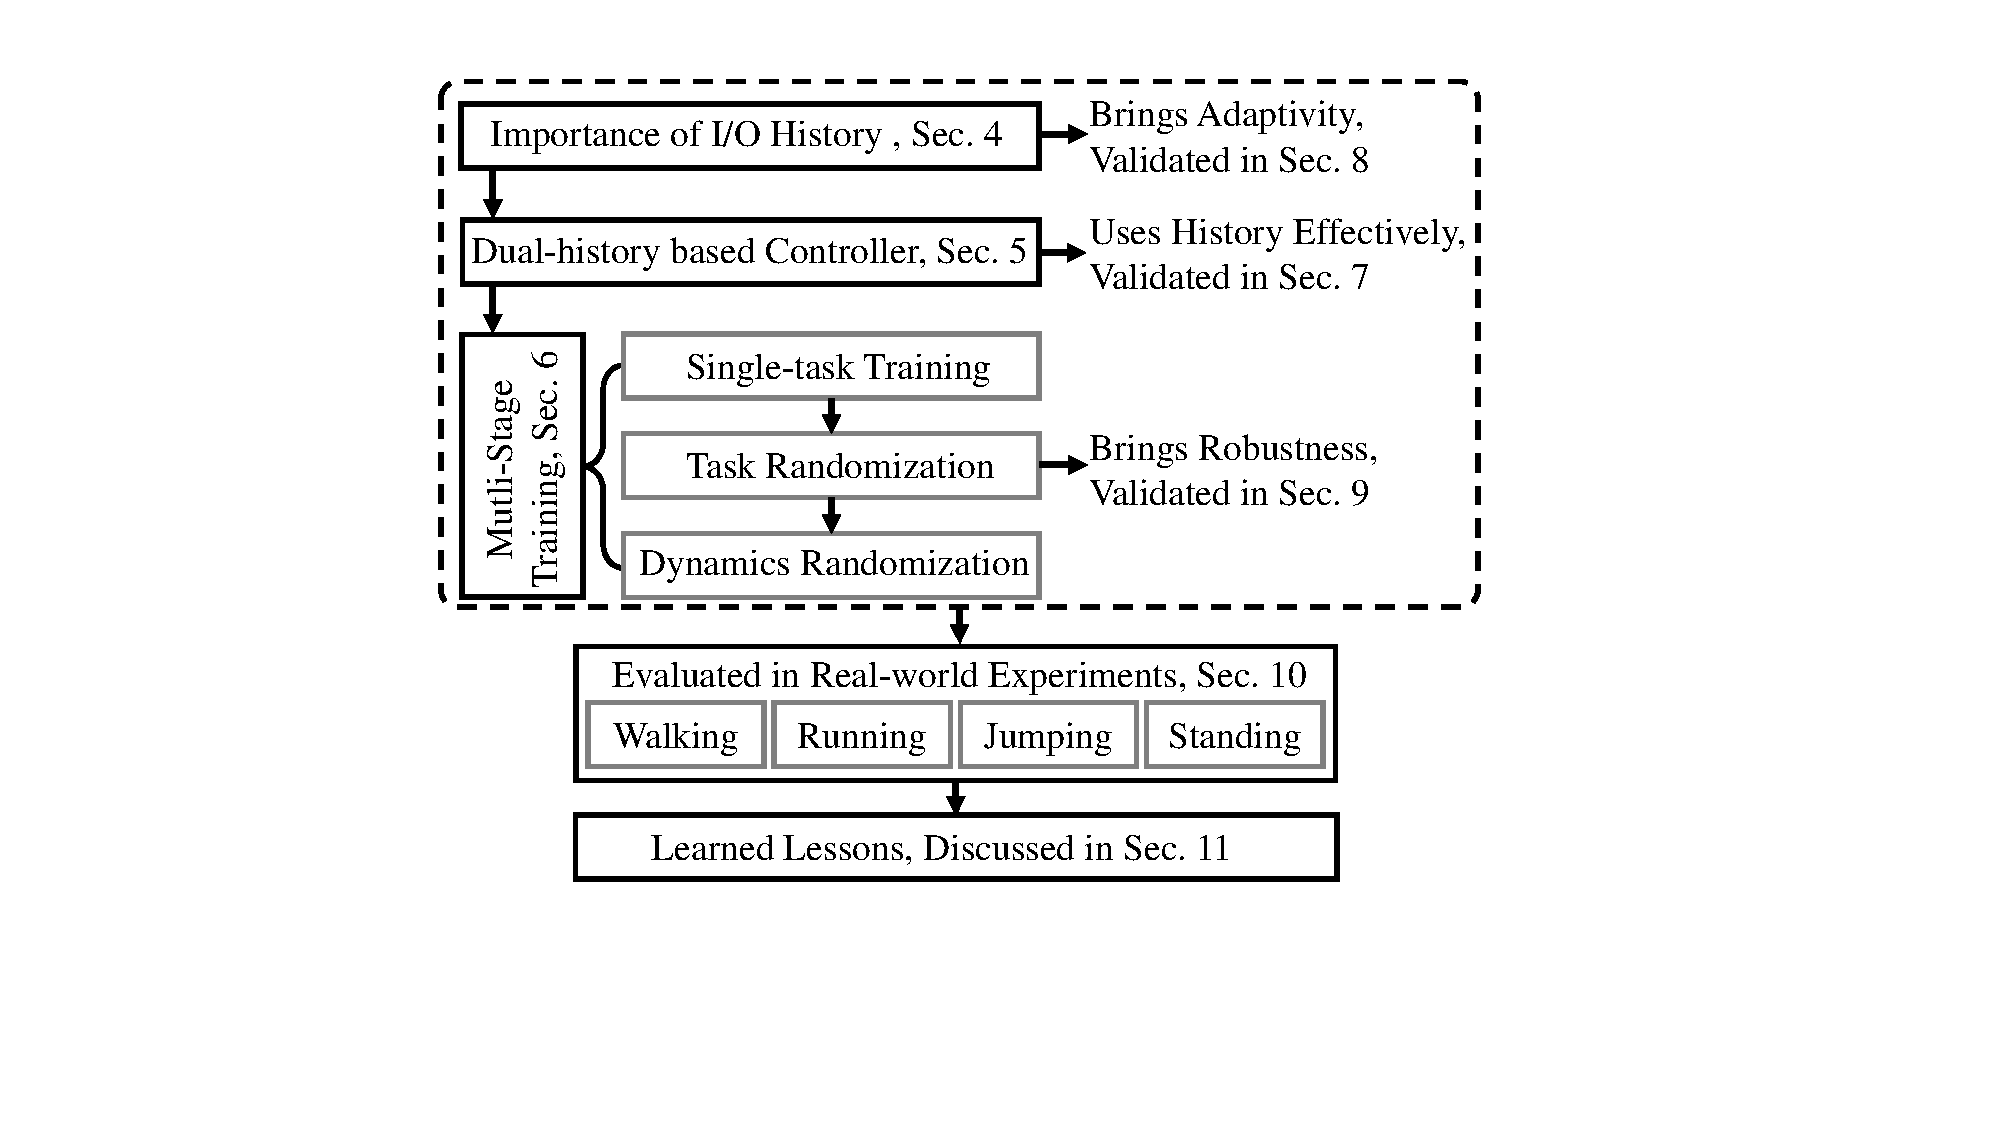
\includegraphics[width=\linewidth]{figures/paper_stucture.pdf}
    \refstepcounter{figure}
    \caption{Overview of this paper. First, Sec.~\ref{sec:background} introduces the formulation of the locomotion control problem and the importance of utilizing the robot's I/O history. The details of our dual-history-based control architecture for various bipedal locomotion skills are presented in Sec.~\ref{sec:controller}, followed by the training scheme discussed in Sec.~\ref{sec:training}. Then, detailed studies are conducted to validate the advantages of the proposed policy structure in Sec.~\ref{sec:policy_structure}, sources of adaptivity in Sec.~\ref{subsec:adaptivity}, and we investigate the sources of the robust behaviors observed in the proposed RL-based controller in Sec.~\ref{sec:multi_skill}. Extensive experiments using the proposed RL-based locomotion controllers to enable Cassie to perform robust standing, walking, running, and jumping skills are presented in Sec.~\ref{sec:experiments}. Insights and discussions for readers interested in applying RL to train bipedal robots are provided in Sec.~\ref{sec:discussion}.}
    \label{fig:overview}
\end{figure}



By using this framework, we obtain skill-specific versatile policies for walking, running, and jumping for a bipedal robot, Cassie. We evaluate the effectiveness of these control policies extensively in the real world in Sec.~\ref{sec:experiments}. 
As we will see, by the adaptivity of the proposed control architecture, the resulting policies can accomplish various tasks with minimal degradation from simulation to the real world and maintain consistency over a long timespan (more than one year). Because of the robustness brought by the proposed training strategy, especially the task randomization, the resulting policies showcase complicated recovery maneuvers when facing unexpected disturbances in the real-time and real world.   
We further summarize the insights and lessons learned during the development of this work in a discussion in Sec.~\ref{sec:discussion}, followed by a conclusion and future work in Sec.~\ref{sec:conclusion}.






